\chapter{Diagramme}
Hier ist eine Auflistung der Diagramme, die für die Arbeit nicht erheblich sind, aber der Verbildlichung von Daten und Unterschieden dienen können.

\begin{figure}[h]
    \centering
    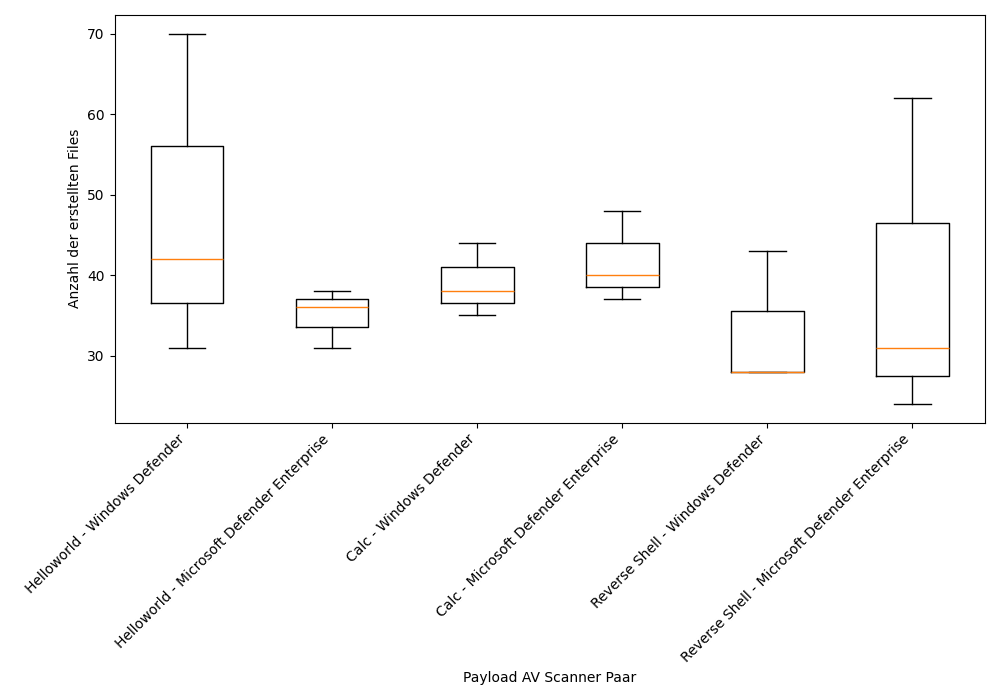
\includegraphics[width=0.85\textwidth]{gfx/Desktriptiv/files_overview.png}
    \caption{Erstellte Files pro Experimente}
    \label{fig:files_overview}
\end{figure}
\begin{figure}[h]
    \centering
    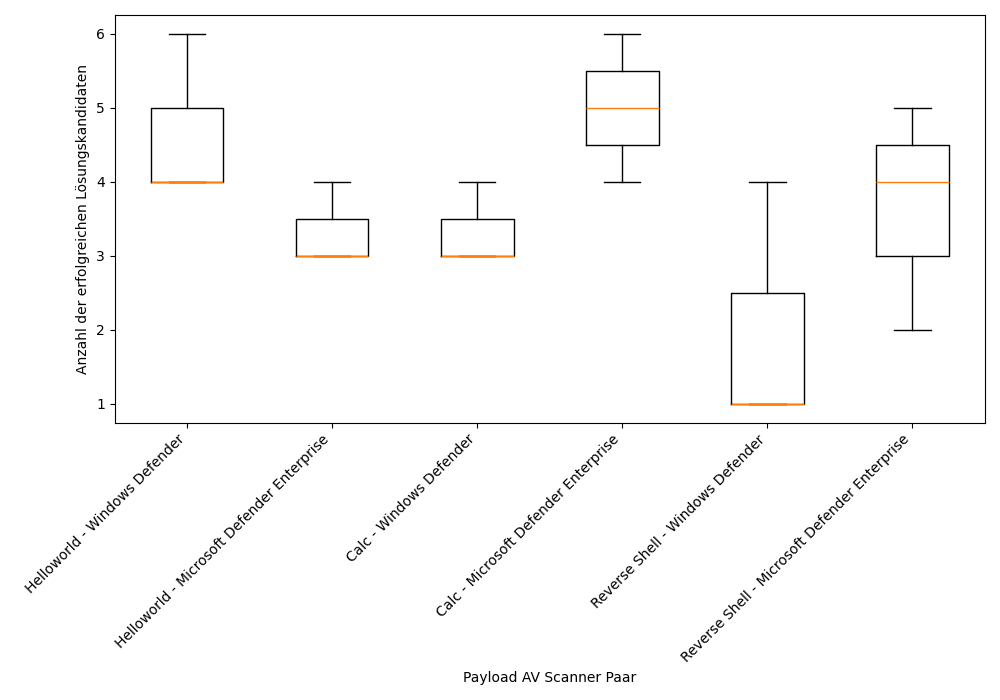
\includegraphics[width=0.85\textwidth]{gfx/Desktriptiv/evaded_overview.png}
    \caption{Anzahl erfolgreicher Obfuskierungen}
    \label{fig:evaded_overview}
\end{figure}
\begin{figure}[]
    \centering
    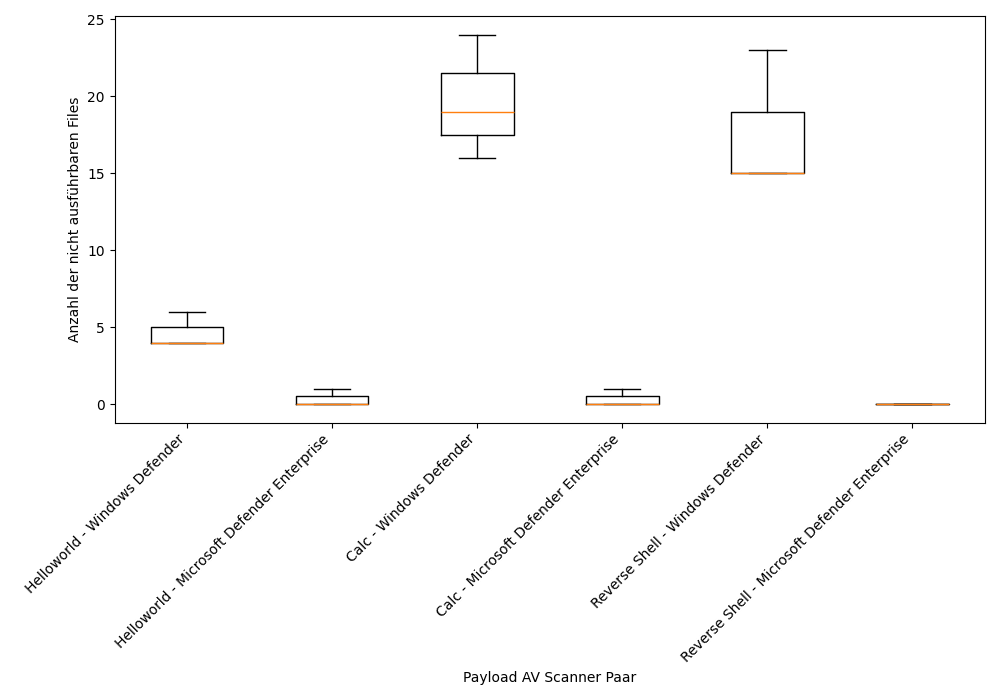
\includegraphics[width=0.85\textwidth]{gfx/Desktriptiv/corrupt_overview.png}
    \caption{Anzahl der Korrupten Dateien}
    \label{fig:corrupt_overview}
\end{figure}
\begin{figure}[h]
    \centering
    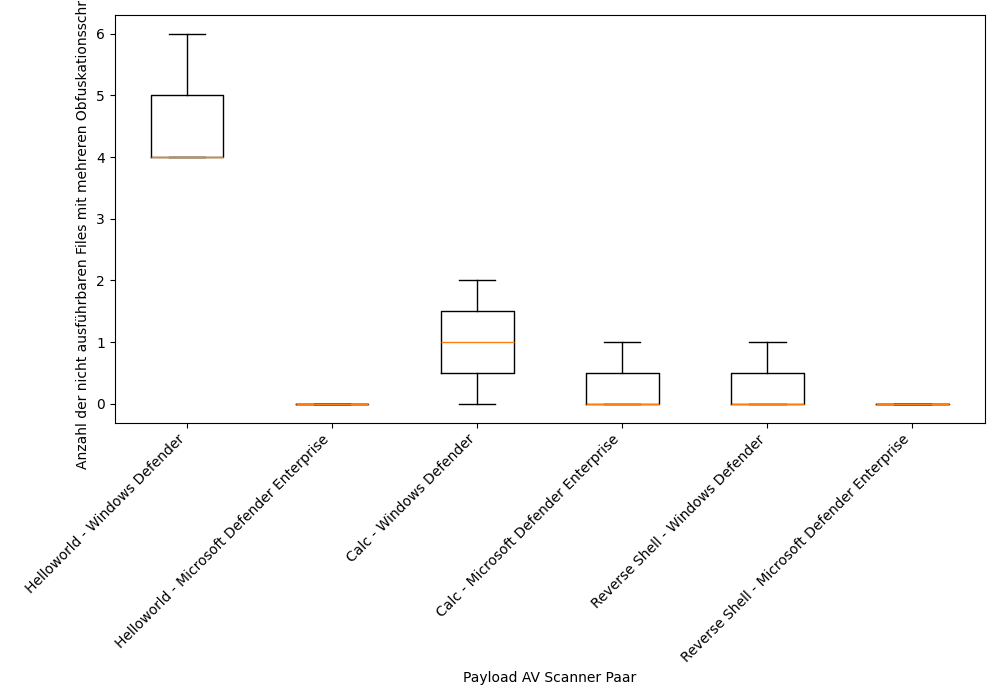
\includegraphics[width=0.85\textwidth]{gfx/Desktriptiv/multicor_overview.png}
    \caption{Anzahl der korrupten, mehrstufigen Obfuskierungen}
    \label{fig:multicor_overview}
\end{figure}